\documentclass[a4paper,12pt,oneside]{report}
\usepackage[utf8]{inputenc}
\usepackage{graphicx}
\usepackage[utf8]{inputenc}
\usepackage[T1]{fontenc}
\usepackage{textcomp}
\usepackage{listings}
\usepackage{hyperref}
\usepackage{xcolor}
\usepackage[nonumberlist]{glossaries}
\definecolor{listinggray}{gray}{0.9}
\definecolor{lbcolor}{rgb}{0.9,0.9,0.9}
\renewcommand{\chaptername}{}
\newcommand{\classname}[1]{\mbox{\textit{\allowbreak #1}}}
\usepackage[ngerman]{babel}
\usepackage{microtype}
\usepackage{lmodern}
\usepackage{longtable}
\usepackage{fancyhdr}
%\usepackage[round]{natbib}
\bibliographystyle{abbrvdin}
\usepackage{wrapfig}
\usepackage{listings}
\setcounter{tocdepth}{3}
\setcounter{secnumdepth}{3}
\lstset{
basicstyle=\footnotesize\ttfamily, % Default font
  % numbers=left,              % Location of line numbers
  numberstyle=\tiny,          % Style of line numbers
  % stepnumber=2,              % Margin between line numbers
  numbersep=5pt,              % Margin between line numbers and text
  tabsize=2,                  % Size of tabs
  extendedchars=true,
  breaklines=true,            % Lines will be wrapped
  keywordstyle=\color{red},
  frame=bt,
  showstringspaces=false,
  % keywordstyle=[1]\textbf,
  % keywordstyle=[2]\textbf,
  % keywordstyle=[3]\textbf,
  % keywordstyle=[4]\textbf,   \sqrt{\sqrt{}}
  stringstyle=\color{blue}\ttfamily, % Color of strings
  showspaces=false,
  showtabs=false,
  xleftmargin=17pt,
  framextopmargin=10pt,
  framexleftmargin=20pt,
  framexrightmargin=20pt,
  framexbottommargin=10pt,
  % backgroundcolor=\color{lightgray},
  showstringspaces=false
}

\makeatletter
\def\@makechapterhead#1{%
  \vspace*{50\p@}%
  {\parindent \z@ \raggedright \normalfont
    \interlinepenalty\@M
    \Huge\bfseries  \thechapter.\quad #1\par\nobreak
    \vskip 40\p@
  }}
\makeatother

\lstdefinelanguage{json}{
    basicstyle=\tiny\ttfamily,
    numbers=left,
    numberstyle=\scriptsize,
    stepnumber=1,
    numbersep=8pt,
    showstringspaces=false,
    breaklines=true,
    frame=lines,
    backgroundcolor=\color{background},
    literate=
     *{0}{{{\color{numb}0}}}{1}
      {1}{{{\color{numb}1}}}{1}
      {2}{{{\color{numb}2}}}{1}
      {3}{{{\color{numb}3}}}{1}
      {4}{{{\color{numb}4}}}{1}
      {5}{{{\color{numb}5}}}{1}
      {6}{{{\color{numb}6}}}{1}
      {7}{{{\color{numb}7}}}{1}
      {8}{{{\color{numb}8}}}{1}
      {9}{{{\color{numb}9}}}{1}
      {:}{{{\color{punct}{:}}}}{1}
      {,}{{{\color{punct}{,}}}}{1}
      {\{}{{{\color{delim}{\{}}}}{1}
      {\}}{{{\color{delim}{\}}}}}{1}
      {[}{{{\color{delim}{[}}}}{1}
      {]}{{{\color{delim}{]}}}}{1},
}

\makeglossaries
\phantomsection
\addcontentsline{toc}{chapter}{Glossar}
\chapter*[Glossar]{Glossar}

\begin{glossary}
    \gls{Python}{Python ist eine Programmiersprache, die sowohl objektorientierte als auch funktionale Programmierung unterstützt. Des Weiteren kann Python als Scriptsprache verwendet werden.}
    \gls{LiDAR}{Steht für \textit{light detection and ranging}. Hierbei werden Laserimpulse ausgesandt und das zurückgestreute Licht detektiert, um Fernmessungen durchzuführen.}
    \gls{Video-Frame}{Ein einzelnes Bild einer Bildsequenz (=Videosequenz).}
    \gls{Odometrie}{Odometrie beschreibt ein Schätzverfahren der Position und Orientierung eines Objektes. Hierbei werden Rückschlüsse aus der Radumdrehung gezogen.}
    \gls{Morphologische Bildverarbeitung}{Beschreibt ein Modell für digitale Bilder, welches auf Verbandstheorie und Topologie basiert. \cite{MM}}
    \gls{Universally Unique Identifier}{Eine als hexadezimal notierte, eindeutige 16-Byte Identifizierungsnummer.}
    \gls{Hex-Farbcode}{Hexadezimale Repräsentation der Rot-, Grün- und Blau-Kanalwerte einer Farbe.}
\end{glossary}


\begin{document}

% Deckblatt >>
\begin{titlepage}
    \begin{center}
        \vspace*{1cm}

        \Huge
        \textbf{Masterthesis}

        \vspace{0.5cm}
        \LARGE
        Simulation und Erprobung verschiedener Szenarien des Autonomen Fahrens am TurtleBot3 

        \vspace{0.75cm}

        \textbf{Moritz Wilke}

        \vspace{0.8cm}

        
\includegraphics[width=0.4\textwidth]{images/host.png}

        \Large
        Hochschule Stralsund\\
        Fakultät für Elektrotechnik und Informatik\\
        \vspace{0.5cm}
        Informatik (INFM)\\
    \end{center}
    \vfill
    \begin{minipage}{0.45\linewidth}
    \begin{flushleft}
       \small
       Erstgutachter:\\
       Prof. Dr. rer. nat. Christian Bunse\\
       \vspace{0.5cm}
       Zweitgutachter:\\
       Dr.-Ing. Jöran Pieper
    \end{flushleft}
    \end{minipage}
    \hfill
    \begin{minipage}{0.45\linewidth}
    \begin{flushright}
      \small
      Matrikel-Nr.:\\
      15214\\
      \vspace{0.5cm}
      Abgabedatum:\\
      06.10.2021
    \end{flushright}
    \end{minipage}
\end{titlepage}
% Deckblatt <<

% Inhaltsverzeichnis >>
\renewcommand{\contentsname}{Inhaltsverzeichnis}
\pagenumbering{gobble}
\tableofcontents
\clearpage
% Inhaltsverzeichnis <<

\pagenumbering{arabic}
\pagestyle{fancy}
\fancyhf{}
\fancyhead[LO]{Hochschule Stralsund - Moritz Wilke}
\fancyhead[CF]{\thepage}
\fancyhead[CH]{}
% Einzelne Kapitel
\chapter{Einleitung}
\fancyhead[RO]{\thechapter. Einleitung}
\section{Motivation}
Das Autonome Fahren ist ein Konzept, welches mehr und mehr an Bedeutung gewinnt. Da mit der zunehmenden
Digitalisierung auch eine höherer Grad der Automatisierung gefragt ist, um z.B. Logistik- oder Transport-Prozesse 
kostengünstiger und sicherer zu gestalten, ergeben sich hierbei auch Anforderungen an das maschinengesteuerte Fahren.
Zum aktuellen Zeitpunkt kommt eine Hybrid-Form in modernen Fahrzeugen bereits zum Einsatz, wodurch unterschiedliche 
Fahrmannöver, wie z.B. das Einparken oder Halten einer Spur, teilautomatisiert werden. Damit das Fahren dauerhaft oder
vollständig von einem Softwaresystem übernommen werden kann, muss es auch in nicht-alltäglichen Situationen nachvollziehbar
entscheiden.

Um zwischen den einzelnen Ebenen der Autonomie zu unterscheiden, werden verschiedene Autonomiestufen definiert.
\begin{itemize}
    \item Autonomiestufe 0: "Driver only", der Fahrer fährt selbst ohne Assistenzsysteme.
    \item Autonomiestufe 1: Der Fahrer wird bei der Bedienung des Fahrezeugs unterstützt, wie z.B. durch einen Tempomat.
    \item Autonomiestufe 2: Das Fahrzeug ist teilautomatisiert und bietet Assistenzsysteme für automatisiertes Einparken 
                            oder zum halten der Spur.
    \item Autonomiestufe 3: Einzelne Fahrmannöver, wie z.B. das Wechseln der Fahrspur, werden vom Fahrzeug automatisiert durchgeführt.
                            Falls Handlungsbedarf für den Fahrer besteht, wird dieser innerhalb einer Vorwarnzeit zur Übernahme
                            der Fahrzeugführung aufgefordert. Aktuell wird darauf hingearbeitet, Fahrzeuge dieser Autonomiestufe
                            für den öffentlichen Straßenverkehr zuzulassen.
    \item Autonomiestufe 4: Das Softwaresystem übernimmt dauerhaft die Steuerung des Fahrzeugs. Falls der Fahrer die Fahrzeugführung
                            übernehmen muss, wird dieser innerhalb einer Vorwarnzeit benachrichtigt.
    \item Autonomiestufe 5: Das Fahrzeug ist vollautomatisiert, ein Fahrer ist nicht länger erforderlich. \cite{BASt}
\end{itemize}

Insbesondere für die Autonomiestufe 3 gab es bereits mehrere Projekte, die solche Systeme in der Praxis getestet haben. Im Juli 2014
gab es hierzu ein Pionierprojekt, bei welchem der Mercedes-Benz Future Truck 2025 auf einem gesperrten Autobahnteilstück bei Magdeburg 
autonom gefahren ist. Das System hat hierbei beispielsweise das mittige Fahren innerhalb der rechten Fahrspur sowie das Beschleunigen
und Bremsen übernommen. Der Fahrer konnte sich somit anderen Aufgaben widmen, wie z.B. der Planung der nächsten Tour oder auch der
Frachtkontrolle über digitale Displays. Durch den Wegfall mehrerer Bedienelemente, hat der Fahrzeugführer in diesem Beispiel auch mehr
Platz im Innenraum. \cite{benz-ft2025}

Zum Erreichen der Autonomiestufe 4 und 5 stellen sich hierbei neben der rechtlichen Grundlage auch technische Herausforderungen.
Ein Beispiel hierfür ist die Erkennung von Wildtieren, die den Straßenverkehr behindern oder gefährden können. Der schwedische
Autohersteller Volvo kann mit seiner Software beispielsweise die heimische Fauna bestehend aus Tieren wie Elchen, Rehen oder Rentieren
zuverlässig erkennen, scheitert jedoch beispielsweise an Kängurus. \cite{volvo-detection-report} 
Dies zeigt, dass es unzählig viele Szenarien gibt, die es beim Autonomen Fahren zu betrachten gibt, um die Fahrsicherheit entsprechend
zu gewährleisten.


\section{Zielstellung}
Welche Szenarien gibt es zu beachten und wie sollen diese bearbeitet werden?


\chapter{Grundlagen}
\fancyhead[RO]{\thechapter. Grundlagen}
\chapter{Grundlagen}
\section{Tools und Frameworks}
\subsection{ROS}
ROS (Robot Operating System) ist ein Framework, mit dem Roboter programmiert werden können. Entgegen dem Namen handelt es sich hierbei nicht um ein Betriebssystem, sondern vielmehr
um eine Middleware. Im Zentrum von ROS stehen einzelne Nodes, welche die Programmlogik beinhalten. Die Nodes kommunizieren über sogenannte Topics mit Nachrichten. Diese Nachrichten
können skalare Datentypen oder komplexe Objekte beinhalten. Eine einzelne Node sendet (=publish) oder empfängt (=subscribe) Nachrichten von einem oder mehreren Topics. Das grundlegende
Paradigma erinnert somit stark an Reactive Programming. Einzelne Nodes lassen sich zur Laufzeit dynamisch starten und stoppen, wodurch eine komplexe, ressourcensparende Programmarchitekur möglich ist.

Die unterstützten Programmiersprachen sind hierbei Python und C++. Hierbei ist es auch möglich, Nodes hybrid mit C++ und Python zu entwickeln. Zusätzlich stehen dem Entwickler mehrere
Bibliotheken zur Verfügung, um die Entwicklung zu vereinfachen. \cite{ROS}

\subsection{Gazebo}
Gazebo ist eine Simulationssoftware, mit der Roboter in komplexen Umgebungen simuliert werden können. Für Gazebo existiert eine Integration für ROS, wodurch es möglich ist,
die Roboter innerhalb einer Simulation über ROS-Nodes zu kontrollieren. Weiterhin gibt es viele bestehende Modelle, welche unter Anderem den TurtleBot 3 repräsentieren, sowie 
vorgefertige Welten, in denen das implementierte Verhalten erprobt werden kann.
Zusätzlich nutzt Gazebo eine Physik-Engine, wodurch Schwerkraft oder Kollisionen berechnet werden, und eine Integration für verschiedenste Sensoren, die auf dem Roboter verbaut sind.
Hierdurch ist es möglich, LiDAR- oder Kameradaten bereits in der Simulation auszuwerten. \cite{Gazebo}

\subsection{TurtleBot 3}
Der TurtleBot 3 ist ein programmierbarer und mobiler Roboter. Grundlegend ist dieser Roboter anpassbar, bringt jedoch im Standard zwei Elektromotoren zur Bewegung, ein 360-Grad-LiDAR-System,
eine Kamera sowie einen Raspberry Pi 3 als Computer mit. Den TurtleBot 3 gibt es in den Ausführungen Burger und Waffle. In der Thesis wird das Modell Burger genutzt. \cite{TurtleBot3}

In Abbildung \ref{fig:TurtleBot3_Burger} ist der TurlteBot 3 Burger zu sehen. Ein weiteres Modell, welches käuflich erwerblich ist, ist der TurtleBot 3 Waffle. Im Rahmen dieser Thesis
wird ausschließlich mit dem TurtleBot3 Burger gearbeitet.

\begin{figure}
  \centering
  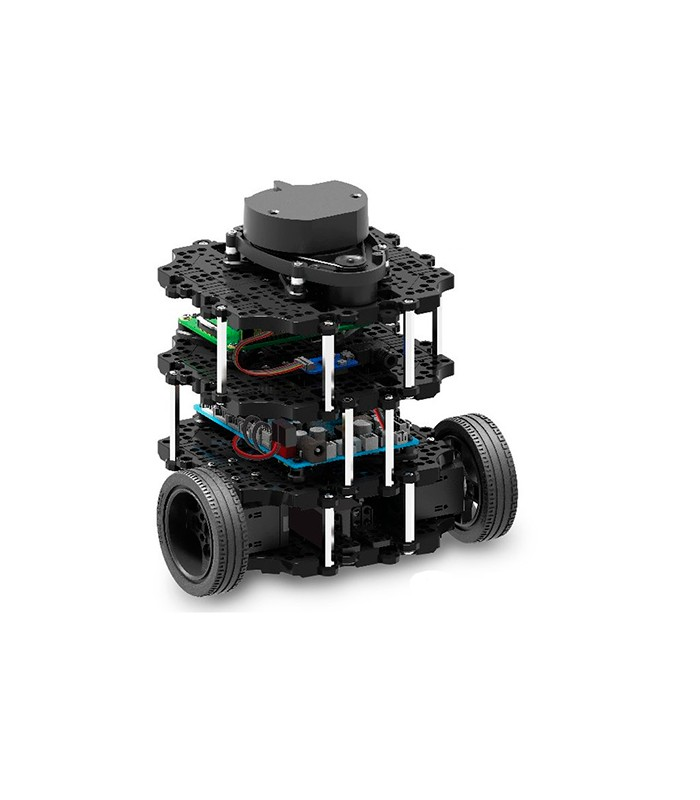
\includegraphics[width=0.4\textwidth]{images/turtlebot-3.jpg}
  \quelle{\url{https://www.roscomponents.com/1326-big_default_2x/turtlebot-3.jpg}}
  \caption{TurtleBot 3 Burger}
  \label{fig:TurtleBot3_Burger}
\end{figure}


\subsection{OpenCV}
OpenCV ist eine Bibliothek, welche Algorithmen und Hilfsfunktionen für die Verarbeitung von Bildern und Videos liefert. Die Bibliothek kann in den Programmiersprachen C, C++, Java und Python genutzt
werden. OpenCV findet hauptsächlich Anwendung in den Feldern Computer Vision und Künstliche Intelligenz.

Grundlegend besteht bei OpenCV die Möglichkeit, ein Video-Frame zu analysieren und zu bearbeiten. Hierdurch besteht die Möglichkeit, Bilder für Folgeprozesse aufzubereiten oder diese
direkt auszuwerten, um beispielsweise Objekte zu erkennen.

\section{Softwaredesign}
Wie bereits erwähnt, wird in dieser Thesis ein bestehendes Projekt aufgegriffen. Somit steht die Wahl der Programmarchitektur nicht frei, sondern wird in die bestehende
Programmarchitektur eingegliedert.

In der bestehenden Architektur gibt es Core-, Detection- und Control-Nodes.
\subsection{Core-Nodes}
In den Core-Nodes werden die Detection- und Control-Nodes dynamisch gestartet und bei Bedarf gestopt. Hierfür werden diverse Topics der Detection-Nodes abonniert, wie z.B. der Erkennung
eines Ampellichts, und bei Bedarf die entsprechende Control-Node gestartet. Zusätzlich wird hier der aktuelle Modus vorgehalten, der beschreibt, ob der Roboter beispielsweise der Fahrspur
folgt oder versucht einzuparken.
Die Core-Nodes sind nicht dafür verantwortlich, Daten zu verarbeiten oder den Roboter zu steuern.

Die bestehende Implementierung beinhaltet zwei Core-Nodes, \ctextit{core\_mode\_decider} und \ctextit{core\_node\_controller}. Die Node \ctextit{core\_mode\_decider} reagiert auf die
Detektion von Verkehrsschildern und wechselt je nach erkanntem Schild den Modus des Roboters. Der Fallback-Modus ist hier in jedem Fall \ctextit{lane\_following} - also die Detektion sowie das 
Fahren in der Fahrspur. Wenn der Roboter ein Schild zum einparken erkennt, wird der Roboter hier beispielsweise in den Modus \ctextit{parking} versetzt. 
Die Node \ctextit{core\_node\_controller} reagiert auf die Veränderung des Modus. Abhängig vom Modus werden hier die Nodes aktiviert oder deaktiviert. 

\subsection{Detection-Nodes}
In den Detection-Nodes werden Sensor- oder Kameradaten sowie die odometrische Position des Roboters ausgewertet. Jede Detection-Node hat eine designierte Aufgabe, wie z.B. das erkennen einer Ampel oder der Fahrspur. Falls das designierte
Objekt erkannt wird, wird ein Nachrichten-Objekt vorbereitet. In diesem Nachrichtenobjekt werden die Daten zusammengefasst, die benötigt werden, um eine entsprechende Entscheidung zu liefern.
Bei der Fahrspurerkennung wird beispielsweise die berechnete Fahrspur-Mitte im Nachrichtenobjekt persistiert. Bei erfolgreicher Detektion wird das Nachrichtenobjekt an ein spezifisches Topic gesendet.

Die bestehende Implementierung beinhaltet sechs Detection-Nodes. Die Nodes, die für die Arbeit Bedeutung haben, sind \ctextit{detect\_lane} und \ctextit{detect\_sign}. Mit der Hilfe von Bildverarbeitungs-Algorithmen
werden hier also die Fahrbahn (\ctextit{detect\_lane}) und verschiedene Verkehrsschilder (\ctextit{detect\_sign}) detektiert.

\subsection{Control-Nodes}
In den Control-Nodes wird der Roboter basierend auf den Erkenntnissen der Detection-Nodes gesteuert. Hierfür abonnieren die Control-Nodes zunächst die Topics der Detection-Nodes.
Falls eine Nachricht empfangen wird, können auf Grundlage dieser Berechnungen durchgeführt werden um den Roboter schlussendlich zu steuern. Diese Steuerung erfolgt in der Regel über
Twistnachrichten, die an andere Topics versendet werden. Diese Twistnachrichten beinhalten Daten, die die lineare und angulare Beschleunigung beschreiben.

Die bestehende Implementierung beinhaltet zwei Control-Nodes. Diese sind \ctextit{control\_lane} und \ctextit{control\_parking}. Lediglich \ctextit{control\_lane} ist im weiteren Verlauf
der Thesis relevant. Hier wird wie bereits beschrieben die Farhbahn-Detektion abonniert. Durch diese wird das Zentrum der Fahrbahn bestimmt. Aus diesem Zentrum wird abgeleitet, wie sehr
angular beschleunigt werden soll.

\section{Simulation}
Für das bestehende Projekt existiert bereits eine Simulation, in der die einzelnen Herausforderungen des TurtleBot AutoRace geprüft werden können. In Abbildung \ref{fig:Autorace_Map}
ist hier der grundsätzliche Aufbau zu sehen. Diese digitale Version dient zum testen und implementieren der Software für den TurtleBot 3 und wurde real nachgebaut. Ein wichtiges
Merkmal ist die Fahrspur, die im Laufe des Projekts beibehalten wurde. Hierbei ist die rechts Fahrbahnbegrenzung weiß (Hex-Farbcode \#ffffff) und die linke Fahrbahnbegrenzung gelb (Hex-Farbcode \#ffff01).
Hierdurch ergibt sich, dass die Fahrbahn nicht bidirektional sondern nur in eine Richtung befahren werden kann.
Am Punkt A in der Abbildung befindet sich der Roboter. Dieser startet mitten in der Fahrbahn und fährt entsprechend der Softwareumsetzung direkt zur ersten Herausforderung am Punkt B.
Punkt B beschreibt die Ampel. Wenn der Roboter sich der Ampel nähert, wird die Ampel von grün auf gelb geschaltet. Die erwünschte Aktion vom Roboter ist, dass dieser langsamer werden soll.
Wenn der Roboter noch näher an die Ampel fährt, wird diese schlussendlich rot. Der Roboter soll nun stehen bleiben, bis die Ampel wieder auf grün schaltet. Nach der Ampel wird das Erkennen und
Einhalten der Fahrspur geprüft, indem Kurven gefahren werden, bis der Roboter an Punkt C ein Parkschild erkennen soll. Bei dieser Herausforderung soll der Roboter automatisch in der freien
Parkfläche ein- und nach erfolgreicher Absolvierung wieder ausparken. Nachdem die Herausforderung abgeschlossen wurde, nähert sich der Roboter der Zollschranke an Punkt D. Hier soll der Roboter
zunächst ein Schild erkennen, welches ihn auf die bevorstehende Aufgabe hinweist. Wenn der Roboter sich in der Nähe der Zollschranke befindet, wird diese heruntergefahren. Der Roboter soll nun
vor der Zollschrank warten, bis diese wieder oben ist. Wenn der Roboter dies geschafft hat, ist die letzte Herausforderung die Navigation durch den Tunnel an Punkt E.
In diesem Tunnel kann die Kamera nicht genutzt werden, da es hier wenig Licht gibt. Der Roboter soll deshalb mit Hilfe des LiDAR-Systems kollisionsfrei durch den Tunnel navigieren.

\begin{figure}[!hbt]
  \centering
  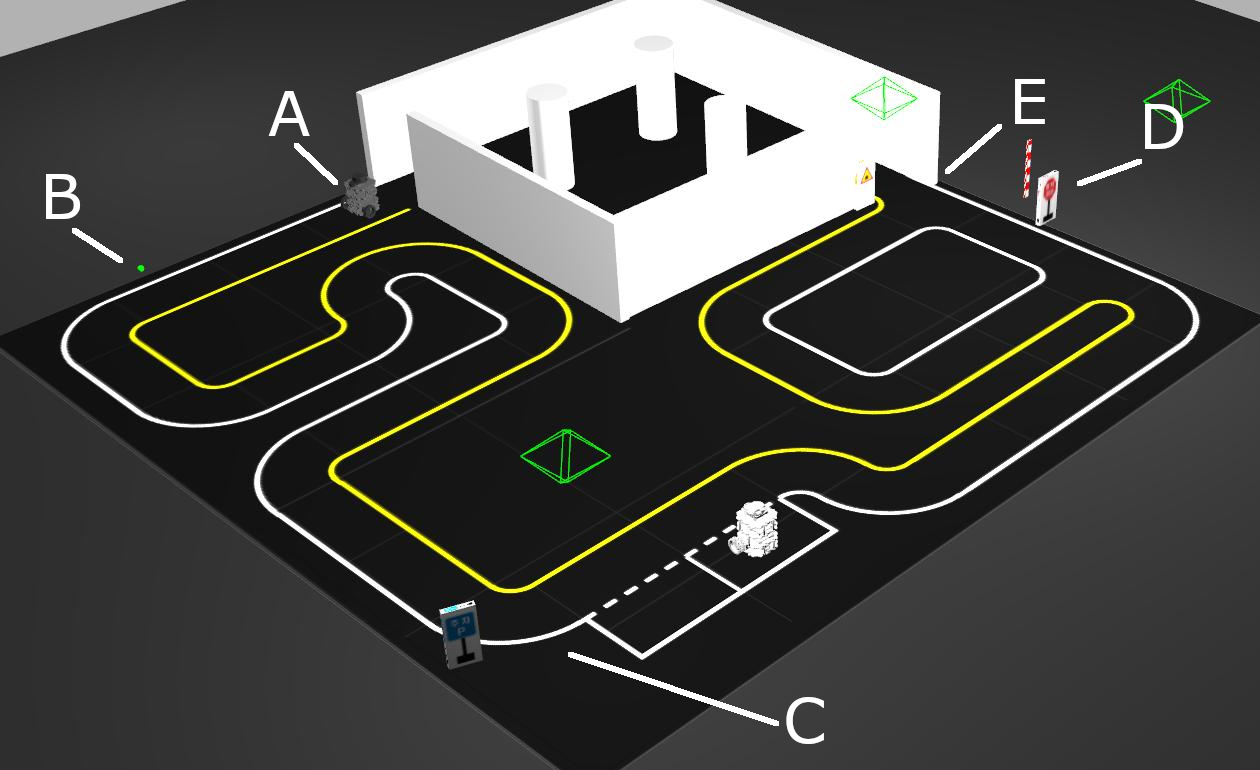
\includegraphics[width=\textwidth]{images/autorace_map.png}
  \quelle{\url{https://emanual.robotis.com/assets/images/platform/turtlebot3/autonomous_driving/autorace_map_mission.png}}
  \caption{Karte des TurtleBot AutoRace 2017}
  \label{fig:Autorace_Map}
\end{figure}

\section{Techniken}
\subsection{Objekterkennung}
Wie bereits erwähnt, sollen in der Arbeit Kreuzungen explorativ erkannt werden. Das bedeutet, dass noch keine Karte oder ähnliches besteht, auf denen alle Kreuzungen aufgelistet sind.
Um eine Kreuzung zu erkennen, ist eine Objekterkennung notwendig, welche auf den Kameradaten des TurtleBot 3 agiert.
\subsubsection{Bildverarbeitung}
Bei der Bildverarbeitung wird auf Grundlage von Bildverarbeitungs-Algorithmen versucht, Erkenntnisse aus Bilddaten zu gewinnen. Hierfür müssen die Bilder in der Regel bereinigt, gefiltert oder transformiert
werden. Bei der Bereinigung ist das Hauptaugenmerk, Rauschen zu unterdrücken. Hierfür können die Bilddaten geglättet, gefiltert oder morphologische Operationen angewendet werden. 
Insbesondere die morphologischen Operationen werden benötigen, um gewisse Strukture oder Figuren, die potenziell durch Bildrauschen beschädigt wurden, zu reparieren.

Bei der Filterung der Bilddaten können diverse Operationen angewendet werden, um Objektstrukturen hervorzuheben oder zu unterdrücken. Ein bekanntes Beispiel ist hier die 
Kantendetektion, die unter Anderem mit dem Sobel-Operator durchgeführt werden kann, welcher unter die Faltungsoperationen fällt. Hierbei wird eine 3x3-Matrix iterativ auf jeden Bildpunkt mit seinen umliegenden Pixeln multipliziert.
Die einzelnen Produkte der Multiplikation werden aufsummiert, um den neuen Grauwert des Pixels vom ursprünglichen Bildpunkt zu berechnen. 
Das Resultat ist hierbei abhängig vom Aufbau der zu verschiebenden Matrix. Der Sobel-Operator G\textsubscript{x} kann beispielsweise genutzt werden, um Vertikale Kanten zu detektieren,
G\textsubscript{y} hingegen wird eher horizontale Kanten herausfiltern. Da die Berechnung der Farbwerte für die Bildpunkte negativ sein kann, können Schwellwerte genutzt werden, um
zu entscheiden, ob ein Pixel Teil einer Kante ist. In Kombination der vertikalen sowie horizontalen Filter mit einem Schwellwert können gute Resultate bei der Kantendetektion erzielt werden. \cite{Sobel}

\[
  G_x=
  \left( {\begin{array}{ccc}
   1 & 0 & -1\\
   2 & 0 & -2\\
   1 & 0 & -1\\
  \end{array} } \right)
\:
  G_y=
  \left( {\begin{array}{ccc}
   1 & 2 & 1\\
   0 & 0 & 0\\
   -1 & -2 & -1\\
  \end{array} } \right)
\]

Der letzte Teil der genutzten Bildverarbeitungsalgorithmen sind die Transformationen. Hierbei können die Bilddaten beispielsweise rotiert oder verschoben werden, um die Perspektive auf das Bild zu verändern.
Ein Beispiel hierfür ist die Rotation, Dehnung oder Translation. Eine Rotation kann zum Beispiel hilfreich sein, wenn die Kamera, die auf ein Fahrzeug montiert ist, eine leichte Schräglage hat.
Somit hätte auch das Urbild, welches bei der Bildverarbeitung analysiert wird, eine Schräglage. Durch eine Rotation entsprechend des Neigungswinkels kann das Bild hierbei korrigiert werden.
Ein Bild kann am Nullpunkt beispielsweise durch Multiplikation mit der Matrix R um den Winkel $\alpha$ rotiert werden.

\[
  R=
  \left( {\begin{array}{cc}
   cos(\alpha) & sin(\alpha)\\
   -sin(\alpha) & cos(\alpha)\\
  \end{array} } \right)
\]

Direkte Algorithmen zur Objekterkennung in Bildern sind z.B. der Marr-Hildreth-Operator (auch Laplacian of Gaussian genannt) oder SIFT (Scale-invariant feature transform) in Kombination
mit einem Feature-Matcher wie FLANN (Fast Library for Approximate Nearest Neighbours). Hierfür ist es notwendig, dass ein Referenzbild vom zu detektierenden Objekt existiert.
Wie bereits beschrieben gibt es eine Node, welche Verkehrsschilder detektiert. Im Hintergrund arbeitet diese Node mit diesem Prinzip. Als Referenzbilder sind hier diverse Verkehrsschilder
hinterlegt. Der Prozess funktioniert vereinfacht beschrieben so, dass beispielsweise über SIFT einzelne Schlüsselpunkte sowohl im Referenzbild als auch im zu verarbeitenden Bild berechnet werden. Im Anschluss
werden die Abweichung bzw. Distanzen zwischen diesen Schlüsselpunkten berechnet. Wenn ausreichend Abweichungen unter einer gewissen Schwelle liegen, ist das Referenzbild im zu verarbeitenden Bild enthalten.
Dieser Ansatz funktioniert recht zuverlässig und kann auch Referenzbilder aus anderen Perspektiven erkennen. Die Kernproblematik hierbei ist jedoch, dass diese Referenzbilder existieren müssen. Für eine
Detektion von Kreuzungen ist dieser Ansatz also nicht geeignet, da eine grenzenlose Menge an Referenzbilder erstellt und geprüft werden müsste.

Bei der Bearbeitung der Thesis wurden weitere Algorithmen eingesetzt. Diese werden an entsprechender Stelle erklärt. Dies hat den Hintergrund, dass die Nutzung und die Auswirkungen der 
Parametrisierung so besser beleuchtet werden kann. Im Kern beruhen diese Algorithmen auf den beschriebenen Prinzipien.

Der Vorteil bei der Nutzung von Bildverarbeitungs-Algorithmen liegt darin, dass die Detektion hierbei auf Strukturen beruht. Solange sich die Strukturen im Kern nicht ändern, kann
das Programm durch eine Anpassung der Parametrisierung an neue Umgebungen angepasst werden. Zusätzlich intigriert sich der Bildverarbeitungs-Ansatz gut in das bestehende Projekt,
da sämtliche existierende Detektionen ebenfalls mit OpenCV umgesetzt wurden.


\subsubsection{Neuronale Netze}
Ein anderer Ansatz zur Erkennung von Objekten ist die Analyse der Bilddaten in einem Neuronalen Netz. Ein solches Netz besteht aus mehreren Neuronen, welche miteinander verbunden sind.
Die einzelnen Neuronen beinhalten hierbei im Regelfall numerische Werte. Die Verbindungen geben hierbei an, wie diese Werte zu wichten sind. Die Eingabedaten werden durch Eingabe-Neuronen
vom Netz ausgewertet. In Ausgabe-Neuronen beinhalten hierbei die Ergebnisse.

Eine spezifische Architektur, um unter Anderem Bilddaten zu verarbeiten, ist das Convolutional Neural Network (CNN). Hierbei wird ein Bild in seine Farbkanäle zerlegt und mit Faltungsalgorithmen,
ähnlich zum beschriebenen Sobel-Operator, verarbeitet. Mit Hilfe von ausreichenden Trainingsdaten, versucht die Maschine selbst die Faltungen zu erkennen, die notwendig sind, um die gewünschten
Ausgaben zu erzielen.

Eine große Herausforderung ist hierbei, das Netz richtig zu konfigurieren. Bei einem Neuronalen Netz gibt es viele Parameter, um die Genauigkeit bei der Verarbeitung der Eingabedaten zu erhöhen, wie z.B.
die Anzahl der Neuronen oder Schichten. Komplexere Parameter beschreiben die Fehlerfunktionen, um Lernfortschritte zu repräsentieren, oder die Aktivierungsfunktion. Die Aktivierungsfunktion
ist dafür zuständig, den Wert vom vorhergehenden, verknüpften Neuron zu verarbeiten.
Durch die Vielfalt an Parametern ist es schwierig, eine zuverlässige Genauigkeit zu erzielen. Jedoch ist es insbesondere beim Autonomen Fahren erstrebsam, eine Genauigkeit von annähernd 100\% zu erreichen,
um Unfälle zu vermeiden.

Aus diesem Grund wird der Ansatz zur Objekterkennung mit einem Neuronalen Netz nicht weiter verfolgt. Eine weitere Problematik ist, dass kein direkter Einfluss darauf genommen werden kann, welche
Faltungen das Netz lernen würde. Somit besteht die Möglichkeit, dass eine Detektion von Kreuzungen ein komplett neues Netz erforder würde, wenn sich beispielsweise die Farbe der Fahrbahn ändert.

Der besondere Vorteil eines neuronalen Netzes wäre, dass es leicht auszuwechseln ist. Dies ist damit begründet, dass die Eingabe- sowie Ausgabe-Neuronen fix sind. Hierdurch würde
das Programm deutlich an Flexibilität gewinnen. Zusätzlich würde sich dieser Ansatz für komplexere Kreuzungen eignen. Das kann bedeuten, dass es dort z.B. verschiedene Fahrspuren
zum abbiegen oder verkehrsregelnde Elemente wie Ampeln gibt. Ein Versuch, der auf einer Kreuzung mit einer Trennung in zwei Straßen aufbaut, wurde bereits im Jahr 1995 durchgeführt \cite{ai-intersection-detection}

\subsection{Connected Cars}
Zur Kommunikation zwischen den Fahrzeugen wird eine Kommunikationsmethode gewählt, die an Connected Cars angelehnt ist. Der Begriff Connected Cars beschreibt grundsätzlich den Datenaustausch
von beispielsweise Positionsdaten mit anderen Verkehrsteilnehmern oder Infrastrukturen, um den Straßenverkehr effizienter und sicherer zu gestalten. Hier kann unter Anderem in folgende Kategorien unterschieden werden:
\begin{itemize}
  \item Vehicle to Vehicle (V2V) - die Fahrzeuge kommunizieren ihre Position und Geschwindigkeit an andere Fahrzeuge
  \item Vehicle to Pedestrian (V2P) - Fahrzeuge und gefährdete Gruppen, wie z.B. Fußgänger oder Radfahrer, kommunizieren ihre Position und Geschwindigkeit untereinander 
  \item Vehicle to Infrastructure (V2I) - Fahrzeuge und Komponenten der Infrastruktur, wie z.B. Ampeln oder Schilder, kommunizieren Daten untereinander
\end{itemize}

Für die Bearbeitung der Thesis ist hierbei insbesondere die V2V-Kommunikation von Bedeutung. Im bestehenden AutoRace-Projekt ist es bereits so, dass ein Roboter
seine odometrischen Daten veröffentlicht. Diese Daten enthalten Angaben zur Position und zur linearen sowie angularen Beschleunigung. Um eine V2V-Kommunikation nachzuahmen,
veröffentlicht jeder Roboter seine odometrischen Daten in einem globalen Topic. Zusätzlich zu den odometrischen Daten enthält veröffentlichte Nachricht einen für jeden Roboter
eindeutigen Universally Unique Identifier (UUID).

\section{Requirements-Engineering}

\subsection{Anforderungsanalyse}
\textit{,,Eine vom Benutzer benötigte Eigenschaft oder Fähigkeit, die eine Software erfüllen oder besitzen muss, um einen Vertrag, einen Standard, eine Spezifikation oder ein anderes formales Dokument zu erfüllen.``} \cite{IEEE610}

Nach IEEE ist dies die Definition einer Anforderung. Nach dieser Definition lassen sich zwei verschiedene Klassen von Anforderungen ableiten. Die Fähigkeiten eines Systems sind hierbei die Funktinalen Anforderungen (FA).
Die Eigenschaften eines Systems hingegen werden von den Nicht-Funktionalen Anforderungen (NFA) repräsentiert.

\subsubsection{Funktionale Anforderungen}
Funktionale Anforderungen werden durch sogenannte Anforderungsquellen identifiziert. Solch eine Anforderungsquelle kann eine Person, ein Prozess in einem Betrieb oder ein Dokument sein.
Insbesondere die Personen, auch oft Stakeholder genannt, sind geeignet, um diverse Problemdomänen zu beschreiben. Anforderungen können darüber hinaus über andere Wege, wie z.B.
Apprenticing oder Feldbeobachten, ermittelt werden.
Eine Möglichkeit, um Funktionale Anforderungen zu beschreiben und zu dokumentieren sind sogenannte Anforderungsschablonen. 
Eine beispielhafte Vorgehensweise hierfür sind ,,Mustergültige Anforderungen - die SOPHIST Templates für Requirements``-Schablonen (MASTeR). \cite{rupp}[S. 219-225]
Über verschiedene Schlüsselwörter kann hierüber eine Anforderung definiert werden. Grundsätzlich baut dieser Prozess auf vier Schritten auf.

\paragraph{Schritt 1}
Es wird festgelegt, wie wichtig die Anforderung ist. Schlüsselwörter hierfür sind ,,Das System \textbf{muss}`` (hohe Priorität) oder aber ,,Das System \textbf{kann}`` (niedrige Priorität).
Bei einer juristisch verbindlichen Anforderung sollte beispielsweise das Modalverb \textbf{muss} eingesetzt werden. ,,Das System muss...`` ist dann das erste Anforderungsfragment.

\paragraph{Schritt 2}
Die geforderte Funktionalität wird identifiziert. Das Zentrum einer jeden Anforderung ist die Funktionalität, die erwünscht ist. Diese Funktionlitäten sind Prozesse, wie z.B. Vorgänge
oder Tätigkeiten. Ein Beispiel hierfür ist ,,Das System muss \textbf{speichern}.``

\paragraph{Schritt 3}
Die Art der geforderten Funktionalität wird festgelegt. Für das Schreiben von Anforderungen sind hierbei drei Systemaktivitäten relevant: Selbsttätige Systemaktivitäten, 
Benutzerinteraktionen und Schnittstellenanforderungen. Aus ,,Das System muss \textbf{speichern}`` wird so beispielsweise ,,A-S-001, Version 1: Selbsttätige Systemaktitivät. Das
System löst eine Backuperstellung aus.``. Anders wäre es, wenn dem Nutzer beispielsweise eine Möglichkeit zur Speicherung gegeben werden würde. Dann würde es eine zusätzliche
Benutzerinteraktions-Anforderung geben.

\paragraph{Schritt 4}
Das Objekt, für welches die Anforderung gefordert wird, muss identifiziert werden. In der definierten Anforderung A-S-001 ist beispielsweise nicht klar, was genau persistiert werden muss.
Besser ist z.B. ,,Das System löst eine Backuperstellung der Kundendaten aus.``

\paragraph{Schritt 5 - optional}
Es wird festgelegt, unter welchen Bedingungen die Funktionalität durchgeführt werden soll. Die vollständige Anforderung könnte dann so aussehen:
,,A-S-001, Version 1: Selbsttätige Systemaktitivät. Wenn es 02:00 Uhr ist, muss das System eine Backuperstellung der Kundendaten auslösen.``

\subsubsection{Nicht-Funktionale Anforderungen}
Bei den Nicht-funktionalen Anforderungen wird zwischen den folgenden Kategorien unterschieden: \cite{rupp}[S. 268]
\begin{description}
\item[Anforderungen an die Benutzeroberfläche:] bündelt Anforderungen zur Beschreibung,
wie sich das System dem Benutzer darstellen soll
\item[Technologische Anforderungen:] schränken den Lösungsraum für die Realisierung dadurch
ein, dass sie Lösungsvorgaben geben oder die Umgebung beschreiben, in der das System betrieben werden soll
\item[Anforderungen an sonstige Lieferbestandteile:] beschreiben alle Produkte, die neben
dem eigentlichen System geliefert werden müssen
\item[Anforderungen an durchzuführende Tätigkeiten:] beschreiben den Entwicklungsprozess
beziehungsweise einzelne, dem Entwicklungsprozess nachgelagerte, Tätigkeiten
\item[Rechtlich-vertragliche Anforderungen:] beschreiben Regelungen zwischen Auftraggeber
und Auftragnehmer
\item[Qualitätsanforderungen:]
Die Qualitätsmerkmale eines Systems sind im Standard ISO25010 \cite{ISO25010} wie folgt definiert:
\begin{itemize}
\item{Functional Suitability (Funktionalität):}
vollständig hinsichtlich Softwarefunktionen, funktional korrekt, angemessene Funktionalität
\item{Reliability (Zuverlässigkeit):}
ausgereifte Softwarequalität, Verfügbarkeit, Fehlertoleranz, Wiederherstellbarkeit
\item{Performance Efficiency (Effizienz):}
Laufzeitverhalten, Ressourcennutzung, Kapazitäten schonen
\item{Compatibility (Kompatibilität):}
Co-Existenz zu weiterer Software, Interoperabilität
\item{Usability (Benutzbarkeit):}
Erkennbarkeit, Erlernbarkeit, Bedienbarkeit, Schutz vor Fehlbedienung, Ästhetische Benutzerschnittstelle, Zugänglichkeit
\item{Maintainability (Wartbarkeit):}
Modularität, Wiederverwendbarkeit, Analysierbarkeit, Modifizierbarkeit, Testbarkeit
\item{Portability (Übertragbarkeit):}
Adaptivität, Installierbarkeit, Austauschbarkeit
\item{Security (Sicherheit):}
Datenschutz, Integrität, nicht manipulierbar, Authentizierbarkeit
\end{itemize}
\end{description}

\subsection{Anforderungsmanagement}
Durch Anforderungsmanagement können einzelne Anforderungen an ein System dokumentiert und nachvollziehbar abgelegt werden. Dies hat den Vortel, dass so zu einem späteren
Zeitpunkt Erkenntnisse darüber gezogen werden können, wie eine einzelne Anforderung und somit auch Änderung im System zustande gekommen ist. Zusätzlich sind Anforderungen
die Grundlage bei der Kommunikation mit Kunden und weiteren Projektbeteiligten. 

Ein Anforderungsmanagement ist also dann relevant, wenn durch die Anforderungen ein System oder Projekt mit hoher Lebensdauer beschrieben wird. Ein anderer Faktor, der für
ein ausgereiftes Anforderungsmanagement sprechen würde, wären mehrere Projektteilnehmer oder eine große Zahl an Anforderungen. \cite[S. 368-372]{rupp}

Da keiner dieser Punkte erfüllt ist, wird auf ein komplexes Anforderungsmanagement verzichtet. Alle Anforderungen an das System werden in dieser Thesis dokumentiert.


\chapter{Konzeption}
\fancyhead[RO]{\thechapter. Konzeption}
\section{Konzeption Szenario 1}
\section{usw...}

\chapter{Simulation}
\fancyhead[RO]{\thechapter. Simulation}
\section{Simulation Szenario 1 (wie geplant, wie Voraussetzung geschaffen, Ziel, Ergebnis usw.)}
\section{usw...}

\chapter{Erprobung}
\fancyhead[RO]{\thechapter. Erprobung}
\section{Erprobung Szenario 1 (wie geplant, wie Voraussetzung geschaffen, Ziel, Ergebnis usw.)}
\section{usw...}

\chapter{Ergebnisse}
\fancyhead[RO]{\thechapter. Ergebnisse}
\input{chapters/6_ergebnisse}

\chapter{Fazit und Ausblick}

\fancyhead[LO]{Hochschule Stralsund - Moritz Wilke}
\fancyhead[CF]{\thepage}
\fancyhead[CH]{}
\fancyhead[RO]{}

\glsaddall
\printglossaries

\bibliography{chapters/literature}

\newpage
\section*{Eidesstattliche Erklärung}
\pagenumbering{gobble}
Ich versichere, die von mir vorgelegte Arbeit selbständig verfasst zu haben. Alle Stellen, die wörtlich oder sinngemäß aus veröffentlichten oder nicht veröffentlichten Arbeiten anderer entnommen sind, habe ich als entnommen kenntlich gemacht. Sämtliche Quellen und Hilfsmittel sind angegeben. Die Arbeit hat mit gleichem bzw. in wesentlichen Teilen gleichem Inhalt noch keiner Prüfungsbehörde vorgelegen.

\vspace{1.5cm}
\begin{flushleft}
\begin{minipage}{0.45\linewidth}
  Stralsund, den ~\hrulefill
\end{minipage}
\hfill
\vspace{0.75cm}
\begin{minipage}{0.45\linewidth}
  \vphantom{Stralsund, den}\hrulefill \\
  Moritz Wilke
\end{minipage}
\end{flushleft}


\end{document}
